\documentclass[11pt]{article}
\usepackage[a4paper,left=3.0cm,right=2.0cm,top=1.0cm,bottom=2.0cm]{geometry}
\usepackage{graphicx}
\usepackage[brazil]{babel}
\usepackage[utf8]{inputenc}
\usepackage{indentfirst}

\author{Eduardo de Araújo Tavares\\Elisson da Silva Melo\\Luciano Serafim de Souza\\Prof.ª Priscilla Vieira}
\title{Universidade Federal Rural de Pernambuco\\Unidade Acadêmica de Garanhuns\\Curso de Bacharelado em Ciência da Computação\vspace{5mm}\\ {\large Projeto da disciplina de Banco de Dados I\\Sistema de gerenciamento de locação de veículos do setor de transportes da Unidade Acadêmica de Garanhuns}}

\begin{document}

\frenchspacing

\maketitle

\begin{abstract}
O SLV - Sistema de Locação de Veículos tem o objetivo de automatizar o processo de solicitação de veículos na Unidade Acadêmica de Garanhuns - UFRPE. Foi inicialmente pensado pelo professor Luciano Souza como solução para o setor de transportes da unidade, uma vez que todo o processo de locação e acompanhamento de locação de veículos para visitas didáticas técnicas e de pesquisa são feitas de forma manual através de planilhas eletrônicas. 
\end{abstract}
\section{Introdução}
O sistema de gerenciamento de locação de veículos consiste em um ambiente onde os usuários poderão solicitar ao setor de transporte a reserva de veículos para realizar atividades referentes a visitação ou pesquisa.

A proposta do sistema é que o usuário tenha a disposição um ambiente WEB e dois aplicativos escritos na linguagem para dispositivos mobile, ANDROID.

O ambiente WEB vai dispor de dois serviços, área administrativa e área do usuário. Ambos terão acesso por meio de cadastro prévio e criação de um login e senha. 

As aplicações para dispositivos mobile vão ser utilizadas pelos usuários (Professores e Técnicos) e motoristas. Poderão ser realizadas solicitações de veículos, acompanhamento de solicitações, cancelamento e preenchimento de relatório de viagem respectivamente.

O sistema terá quatro tipos de usuário, 'Administrador' (Funcionário responsável pelo Setor de Transportes), 'Técnico' (Servidores em geral da Instituição), 'Professor Pesquisador (Professores que desenvolvam atividades de pesquisa e que precise locar carro destinado para esse fim) e 'Professor' (Professor que não desenvolve atividade de pesquisa, mas precisará de veículos para desenvolver atividades de práticas e visitação). Esses últimos serão cadastrados por Administradores levando-se em conta os dados necessários para a correta identificação dos mesmos, incluindo-se documentos e dados institucionais. Como citado acima ambos os tipos de usuário possuirão credenciais para login no sistema.

Após o login, o usuário terá acesso à sua área onde poderá preencher um formulário para a solicitação de veículos. Ao término da solicitação será gerado um número de protocolo e o pedido seguirá para análise pelo setor responsável. O usuário poderá verificar o status de seus pedidos em andamento buscando-os pelo protocolo ou através da visualização dos pedidos associados a seu nome ou matrícula, havendo também a possibilidade de cancelamento do pedido.

Será possível aos Administradores consultar todos os dados do sistema. Caberá a eles a inclusão ou exclusão de veículos e usuários do sistema, assim como a alteração de status dos pedidos. Para definir um status como 'Concluído', será necessário a entrada dos dados quantitativos referentes à viagem, incluindo o número de quilômetros rodados e quantidade de combustível consumido.

O objetivo deste projeto é o de automatizar a alocação de veículos na instituição, facilitando a atividade que hoje vem sendo feita através de planilhas eletrônicas e formulários preenchidos a cunho.

\section{MER - Modelo Entidade Relacionamento}
Pode-se ver abaixo o Modelo Entidade Relacionamento. Aqui são descritos em forma de diagrama as entidades envolvidas e os relacionamentos entre elas.
\begin{center}
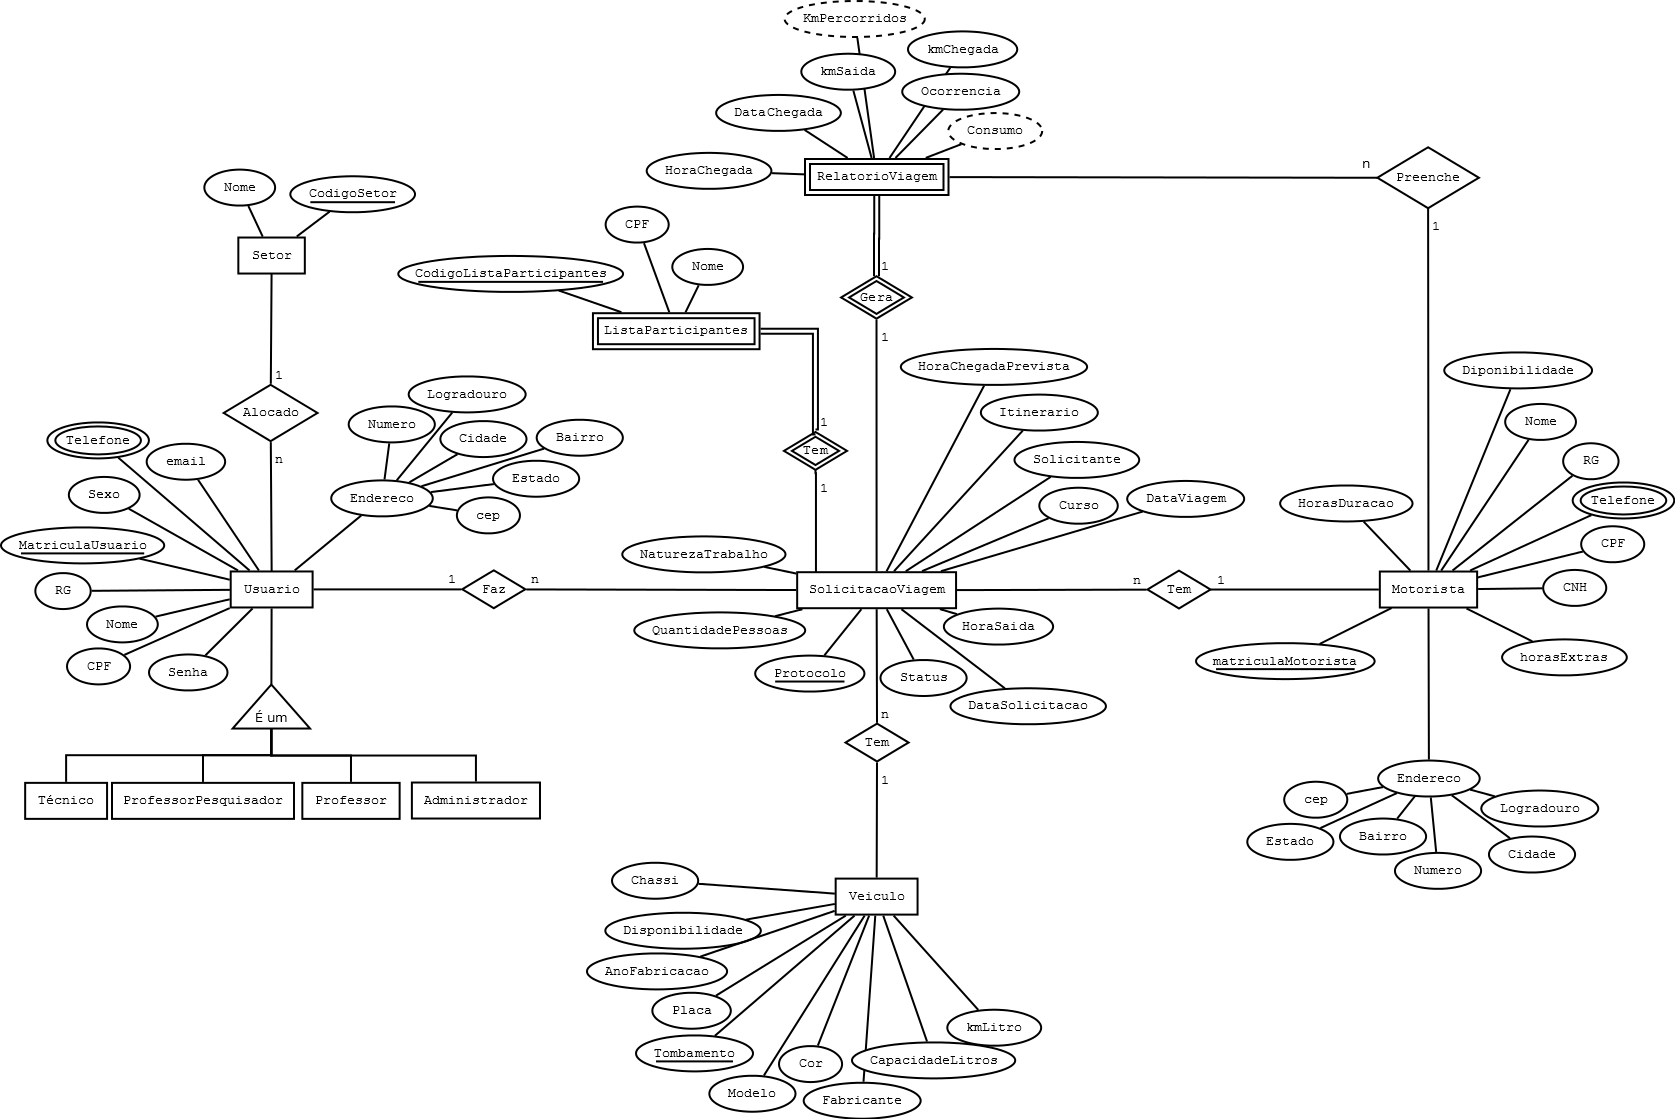
\includegraphics[scale=0.25]{esquema.png}
\end{center}   

\subsection{Dicionário de dados}
Descreveremos agora cada entidade e seus atributos de acordo com seu papel dentro do sistema.
\begin{table}[htp]\centering
\begin{tabular}{|l||l|}
\hline
Atributo & Descrição \\ \hline \hline
Nome &  \\ \hline
CPF &  \\ \hline
RG &  \\ \hline
MatriculaUsuario &  \\ \hline
\end{tabular}
\caption{usuario}
\end{table}

\subsection{Modelo Esquema Relacional}

\subsubsection{Entidades regulares}
\begin{itemize}
\item usuario(\underline{matriculaUsuario}, nome, rg, cpf, senha,
email, sexo, logradouro, numero, cidade, bairro, estado, cep)

\item setor(\underline{codigoSetor}, nome)

\item solicitacaoViajem(\underline{protocolo}, solicitante, horaSaida, horaChegadaPrevista, dataViajem, naturezaTrabalho, quantidadePessoas, status, curso, itinerario, DataSolicitacao)

\item Motorista(\underline{matriculaMotorista}, rg, cpf, cnh, nome, disponibilidade, logradouro, numero, cidade, bairro, estado, cep)

\item veiculo(\underline{tombamento}, fabricante, modelo, cor, placa, anoFabricacao, chassi, disponibilidade, capacidadeLitros, kmLitro)
\end{itemize}

\subsubsection{Entidades Fracas}
\begin{itemize}

\item historico(\underline{codigoHistorico}, protocolo, kmSaida, kmChegada, dataChegada, horaChegada, ocorrencia)

\end{itemize}

\subsubsection{Relacionamentos 1:1}
\begin{itemize}

\item Como a entidade fraca ,Historico, também tem cardinalidade 1:1 e na regra anterior já foi tradado nesse passo não será necessário faze-lo.
\end{itemize}

\subsubsection{Relacionamentos 1:n(Que não envolvem entidades fracas)}
\begin{itemize}

\item usuarios(\underline{matriculaUsuario}, codigoSetor, nome, rg, cpf, senha,
email, sexo, logradouro, numero, cidade, bairro, estado, cep)

\item solicitacaoViajem(\underline{protocolo}, solicitante, horaSaida, horaChegadaPrevista, dataViajem, naturezaTrabalho, quantidadePessoas, status, curso, itinerario, DataSolicitacao, matriculaUsuario, tombamento, matriculaMotrista)

\end{itemize}

\subsubsection{Relacionamentos n:m}
Não existe relacionamento n:m.

\subsubsection{Atributos multivalorados}
\begin{itemize}

\item telefone(\underline{codigoTelefone}, matriculaUsuario, matriculaMotorista, numeroResid, numeroCel)

\end{itemize}

\subsubsection{Especialização e Generalização}

\begin{itemize}

\item usuarios(\underline{matriculaUsuario}, codigoSetor, identificador, nome, rg, cpf, senha,
email, sexo, logradouro, numero, cidade, bairro, estado, cep)

\end{itemize}

\section{Normalização}
Dado que o processo de modelagem para o esquema er foi eficaz, a normalização não foi necessária.

\section{Esquemas definitivos}
\begin{itemize}

\item usuarios(\underline{matriculaUsuario}, codigoSetor, identificador, nome, rg, cpf, senha, email, sexo, logradouro, numero, cidade, bairro, estado, cep)

\item telefone(\underline{codigoTelefone}, matriculaUsuario, matriculaMotorista, numeroResid, numeroCel)

\item solicitacaoViajem(\underline{protocolo}, solicitante, horaSaida, horaChegadaPrevista, dataViajem, naturezaTrabalho, quantidadePessoas, status, curso, itinerario, DataSolicitacao, matriculaUsuario, tombamento, matriculaMotrista)

\item veiculo(\underline{tombamento}, fabricante, modelo, cor, placa, anoFabricacao, chassi, disponibilidade, capacidadeLitros, kmLitro)

\item historico(\underline{codigoHistorico}, protocolo, kmSaida, kmChegada, dataChegada, horaChegada, ocorrencia)

\item setor(\underline{codigoSetor}, nome)

\item Motorista(\underline{matriculaMotorista}, rg, cpf, cnh, nome, disponibilidade, logradouro, numero, cidade, bairro, estado, cep)

\end{itemize}

\section{Funcionalidades}
\subsection{Administrador}
\begin{enumerate}
\item Cadastrar usuarios
\item Cadastrar setor
\item Cadastrar motorista
\item Cadastrar veículo
\item Alterar usuarios
\item Alterar setor
\item Alterar motorista
\item Alterar veículo
\item Modificar status
\item Finalizar Solicitação
\end{enumerate}

\subsection{Usuário}
\begin{enumerate}
\item Solicitar viagem
\item Consultar status
\end{enumerate}

\section{Scripts SQL}

\begin{verbatim}
CREATE DATABASE location;
USE location;
CREATE TABLE motorista (
matriculaMotorista CHAR(11) NOT NULL,
rg CHAR(7) NOT NULL,
cpf CHAR(11) NOT NULL,
cnh CHAR(11) NOT NULL,
nome VARCHAR(80) NOT NULL,
sexo CHAR(1) NOT NULL,
horasExtras INT DEFAULT 0 NOT NULL,
disponibilidade BOOLEAN DEFAULT 0 NOT NULL,
logradouro VARCHAR(80) NOT NULL,
numero VARCHAR(5) NOT NULL,
cidade VARCHAR(45) NOT NULL,
bairro VARCHAR(45) NOT NULL,
estado CHAR(2) NOT NULL,
cep CHAR(8) NOT NULL,
PRIMARY KEY (matriculaMotorista)
);

CREATE TABLE setor (
codigoSetor INT AUTO_INCREMENT NOT NULL,
nome VARCHAR(80) NOT NULL,
PRIMARY KEY (codigoSetor)
);

CREATE TABLE veiculo (
tombamento VARCHAR(20) NOT NULL,
chassi VARCHAR(120) NOT NULL,
disponibilidade BOOLEAN DEFAULT 0 NOT NULL,
anoFabricacao CHAR(4) NOT NULL,
placa CHAR(7) NOT NULL,
cor VARCHAR(20) NOT NULL,
fabricante VARCHAR(40) NOT NULL,
capacidadeLitros CHAR(3) NOT NULL,
kmLitros CHAR(2) NOT NULL,
PRIMARY KEY (tombamento)
);

CREATE TABLE usuario (
matriculaUsuario CHAR(11) NOT NULL,
nome VARCHAR(80) NOT NULL,
rg CHAR(7) NOT NULL,
cpf CHAR(11) NOT NULL,
sexo CHAR(1) NOT NULL,
email VARCHAR(80) NOT NULL,
identificador VARCHAR(30) NOT NULL,
senha VARCHAR(8) NOT NULL,
codigoSetor INT NOT NULL,
logradouro VARCHAR(80) NOT NULL,
numero VARCHAR(5) NOT NULL,
cidade VARCHAR(45) NOT NULL,
bairro VARCHAR(45) NOT NULL,
estado CHAR(2) NOT NULL,
cep CHAR(8) NOT NULL,
PRIMARY KEY (matriculaUsuario)
);

CREATE TABLE telefone (
codigoTelefone INT AUTO_INCREMENT NOT NULL,
numeroResid CHAR(11) NOT NULL,
numeroCel CHAR(11) NOT NULL,
matriculaUsuario CHAR(11),
matriculaMotorista CHAR(11),
PRIMARY KEY (codigoTelefone)
);

CREATE TABLE solicitacaoViajem (
protocolo BIGINT AUTO_INCREMENT NOT NULL,
status INT DEFAULT 0 NOT NULL,
naturezaTrabalho VARCHAR(256) NOT NULL,
quantidadePessoas CHAR(3) NOT NULL,
horaSaida TIME NOT NULL,
horaChegadaPrevista TIME NOT NULL,
itinerario VARCHAR(256) NOT NULL,
solicitante VARCHAR(80) NOT NULL,
curso VARCHAR(80) NOT NULL,
horaDuracao TIME NOT NULL,
dataViajem DATE NOT NULL,
dataSolicitacao DATE NOT NULL,
matriculaUsuario CHAR(11) NOT NULL,
tombamento CHAR(20) NOT NULL,
matriculaMotorista CHAR(11) NOT NULL,
PRIMARY KEY (protocolo)
);

CREATE TABLE historicoViajem (
codigoHistorico INT AUTO_INCREMENT NOT NULL,
kmSaida NUMERIC(6,2),
kmChegada NUMERIC(6,2),
dataChegada DATE,
ocorrencia VARCHAR(256),
horaChegada TIME,
protocolo BIGINT NOT NULL,
PRIMARY KEY (codigoHistorico)
);

ALTER TABLE solicitacaoViajem ADD CONSTRAINT motorista_solicitacaoviajem_fk
FOREIGN KEY (matriculaMotorista)
REFERENCES motorista (matriculaMotorista)
ON DELETE NO ACTION
ON UPDATE NO ACTION;

ALTER TABLE telefone ADD CONSTRAINT motorista_telefone_fk
FOREIGN KEY (matriculaMotorista)
REFERENCES motorista (matriculaMotorista)
ON DELETE NO ACTION
ON UPDATE NO ACTION;

ALTER TABLE usuario ADD CONSTRAINT setor_usuario_fk
FOREIGN KEY (codigoSetor)
REFERENCES setor (codigoSetor)
ON DELETE NO ACTION
ON UPDATE NO ACTION;

ALTER TABLE solicitacaoViajem ADD CONSTRAINT veiculo_solicitacaoviajem_fk
FOREIGN KEY (tombamento)
REFERENCES veiculo (tombamento)
ON DELETE NO ACTION
ON UPDATE NO ACTION;

ALTER TABLE solicitacaoViajem ADD CONSTRAINT usuario_solicitacaoviajem_fk
FOREIGN KEY (matriculaUsuario)
REFERENCES usuario (matriculaUsuario)
ON DELETE NO ACTION
ON UPDATE NO ACTION;

ALTER TABLE telefone ADD CONSTRAINT usuario_telefone_fk
FOREIGN KEY (matriculaUsuario)
REFERENCES usuario (matriculaUsuario)
ON DELETE NO ACTION
ON UPDATE NO ACTION;

ALTER TABLE historicoViajem ADD CONSTRAINT solicitacaoviajem_historicoviajem_fk
FOREIGN KEY (protocolo)
REFERENCES solicitacaoViajem (protocolo)
ON DELETE NO ACTION
ON UPDATE NO ACTION;

\end{verbatim}

\section{Consultas}

\begin{enumerate}
\item Liste todos os usuários seus telefones e setor onde estão alocados. 
\begin{verbatim}
SELECT u.matriculaUsuario, u.nome, s.nome, t.numeroResid, 
t.numeroCel, logradouro, numero, cidade,bairro, estado,cep
FROM usuario u, setor s, telefone t
WHERE u.codigoSetor = s.codigoSetor
AND u.matriculaUsuario = t.matriculaUsuario
\end{verbatim}

\item Liste todos os motoristas e seus telefones. 
\begin{verbatim}
SELECT m.matriculaMotorista, m.nome,t.numeroResid,
t.numeroCel,logradouro,numero, cidade,bairro,estado,cep
FROM motorista m, telefone t
WHERE m.matriculaMotorista = t.matriculaMotorista
\end{verbatim}

\item Liste todas as solicitações de viagem do usuario com matricula Y e data entre W e Z. 
\begin{verbatim}
SELECT protocolo, matriculaUsuario,
solicitante, dataSolicitacao, curso,
naturezaTrabalho 
FROM solicitacaoViajem 
WHERE matriculaUsuario = 'Y' dataSolicitacao BETWEEN 'W'AND 'Z'
\end{verbatim}

\item Liste as solicitações e seus históricos. 
\begin{verbatim}
select x.protocolo, x.matriculaUsuario, x.solicitante, 
x.curso, x.dataSolicitacao, 
x.dataViajem, x.matriculaMotorista, 
x.nomeMotorista, x.horaSaida, h.horaChegada, h.ocorrencia
from historicoViajem h left join 
(select s.protocolo, s.matriculaUsuario, s.solicitante, 
s.curso, s.dataSolicitacao,s.dataViajem, s.matriculaMotorista, 
m.nome as nomeMotorista, s.horaSaida 
from solicitacaoViajem s, motorista m 
where s.matriculaMotorista = m.matriculaMotorista) 
x on x.dataSolicitacao between '20140101' and '20140501';
\end{verbatim}
\end{enumerate}

\section{Ferramentas}
Serão utilizadas as seguintes ferramentas para o desenvolvimento do projeto:
\begin{itemize}
\item IDE Netbeans 7.4
\item Banco de Dados Mysql
\item SGBD: Mysql WorkBench
\item Framework gráfico Primefaces
\item Servidor de aplicação GlassFish
\end{itemize}
\end{document}
